\documentclass[10pt,a4paper]{article}
\usepackage[T1]{fontenc}
\usepackage[utf8]{inputenc}
\usepackage[margin=25mm]{geometry}
\usepackage{lmodern,microtype}
\usepackage{graphicx,booktabs,adjustbox}
\usepackage[dvipsnames]{xcolor}
\usepackage{tikz}
\usetikzlibrary{arrows.meta,positioning}
\usepackage[numbers,sort&compress]{natbib}
\usepackage[hidelinks]{hyperref}
\usepackage{enumitem}
\usepackage[section]{placeins}
\setlist{nosep}
\setlength{\emergencystretch}{2em}
\newcommand{\pending}[1]{\textcolor{BrickRed}{\textbf{[pending]}}}
\newcommand{\resulttable}[1]{\begin{adjustbox}{max width=\linewidth}\input{results/#1}\end{adjustbox}}
\title{Auto-Assessment: Rubric-Grounded Grading of Handwritten Answer Sheets with Red-Ink Feedback}
\author{Basavaraj A Naduvinamani (DA25C005)\\DA7016, IIT Madras}
\date{}
\begin{document}
\maketitle
\begin{abstract}
Auto-Assessment grades answer sheets against a teacher's rubric and returns evidence-linked marks, feedback and red-ink annotations. We evaluate typed SPRAG responses and a handwritten classroom set, distinguishing grading from end-to-end document reading. On SPRAG test, advocate-only review achieves quadratic weighted kappa (QWK) 0.723 [0.667, 0.773], mean absolute error (MAE) 0.85 of 5 and within-1 agreement of 76\%, compared with lexical-baseline QWK 0.375 and human--human QWK 0.962. The review ablation finds that a critic permitted only to lower marks increases negative bias; advocate-only was selected on development data for MAE and near-zero bias. Confidence gating on the full pipeline accepts 62\% of answers at MAE 0.66, while the selected configuration accepts 92\% at MAE 0.76. On handwritten classroom answers, QWK against a single teacher is 0.47 [0.32, 0.57]. A targeted injection check reveals score manipulation despite prompt-level safeguards; a wording-specific pattern subsequently routes matching answers to a teacher. A Hindi worked example demonstrates the translation path without claiming multilingual evaluation. The remaining gap to human agreement supports selective auto-marking with teacher review, rather than autonomous replacement of examiners.
\end{abstract}
\section{Introduction}
Marking an exam booklet requires more than assigning a total. A teacher must associate each response with a question, recognise partial understanding, justify deductions and decide when an uncertain answer needs another look. Handwriting and multilingual text add recognition and interpretation errors before a marking decision is made. A fluent explanation is insufficient if it cannot be traced to the student's work or the teacher's rubric.

Auto-Assessment treats the rubric as an explicit contract. It accepts an exam specification containing questions, criterion descriptions and model answers, together with typed sheets, scans or photographs. It returns criterion marks, verbatim evidence, actionable feedback, an HTML report and a red-ink annotated booklet. The intended role is selective auto-marking with teacher review, preserving an inspectable basis for both credit and referral.

This report evaluates that role on typed SPRAG responses and a small real handwritten classroom set. The central analytical question is whether review mechanisms improve agreement or merely change its direction. An advocate can recover missed credit; a strict critic can only remove it. The ablation finds that the critic increases under-marking, motivating an advocate-only default chosen on development data. A separate confidence analysis asks how much marking can be accepted automatically at a stated error level.

The contributions are an integrated full-sheet workflow with evidence checks and bounded awards; an empirical comparison of review directions; a confidence-based referral mechanism; and a report that distinguishes typed grading, handwritten end-to-end performance and targeted injection checks. Feedback remains the educational motivation, but its quality has not yet been rated by students and no learning effect is claimed. The measurements support assisted marking within the tested settings, rather than a validated replacement for teachers.

\section{Related work}
\subsection{Language models as judges and short-answer graders}
The use of language models as judges motivates both the flexibility and the risks of this design. Zheng et al.\ study model-based evaluation of conversational responses and discuss biases in model judgements \citep{zheng2024judging}. That setting differs from exam marking: an educational rubric assigns credit to specific demonstrated ideas, and a plausible response can still contain a factual error. The present system therefore constrains model output with criterion identifiers, mark bounds and evidence checks instead of treating a generated score as self-validating.

Automated short-answer grading also predates current generative models. Mohler et al.\ use semantic similarity and dependency-graph alignment to connect student responses to reference answers \citep{mohler2011learning}. This provides a useful distinction between lexical overlap and the meaning of an answer. Auto-Assessment retains a lexical baseline as a deliberately limited reference point. Its scripted offline provider similarly tests control flow rather than semantic judgement; successful dry runs are not evidence that the language-model grader understands an answer.

\subsection{Indic OCR and handwritten documents}
The implementation integrates Bodhan's hosted IndicOCR interface, local IndicOCR weights and precomputed OCR JSON, with provider adapters converting results to common page and line contracts. The local adapter retains reading order, boxes, confidence and block kinds where available. The combination of page layout and text recognition is relevant to scripts with multiple questions, equations and mixed writing systems.
% TODO cite: verify a primary Bodhan / AI4Bharat IndicOCR publication or model card before adding a bibliographic claim.
No OCR benchmark result is imported from the archived project report. Language coverage advertised by a provider must be distinguished from accuracy on the project's own handwriting and scanning conditions. This report evaluates the latter only when paired scans and transcripts are available.

\subsection{Selective prediction}
Selective classification formalises a system's ability to abstain rather than answer every input, and examines the trade-off between coverage and risk \citep{geifman2017selective}. Auto-Assessment adopts that operational perspective: the teacher should see how accurate the automatically accepted subset is and how much work remains for manual review. Its confidence is a minimum of diagnostic signals, not a calibrated probability of correctness. A coverage curve can assess the usefulness of that heuristic, but cannot by itself establish fairness or eliminate systematic errors shared by the graders.

\section{System}
\label{sec:system}
The package separates provider interfaces from grading logic. A teacher-authored exam specification is validated before use, and typed data contracts connect the stages. Figure~\ref{fig:pipeline} shows the principal processing order. The same grading pipeline supports the command line and HTTP API; the interactive demonstration adds file upload and marked-booklet presentation.

\begin{figure}[htbp]
\centering
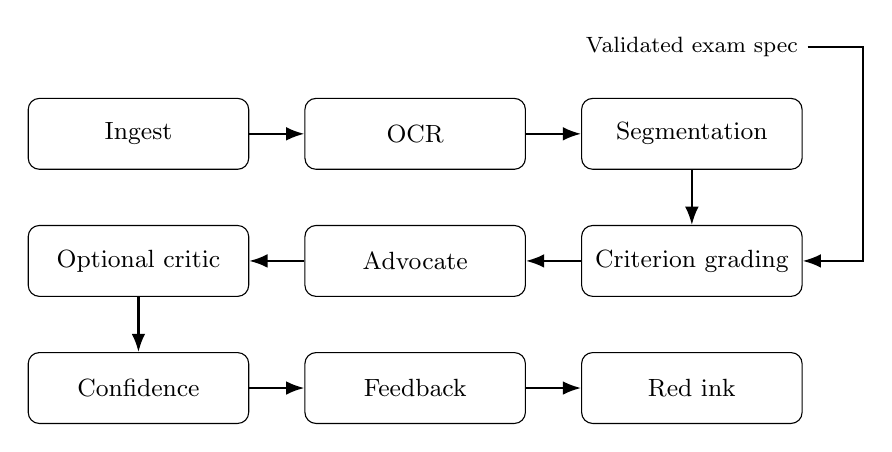
\begin{tikzpicture}[
  stage/.style={draw,rounded corners,align=center,minimum width=28mm,minimum height=9mm,font=\small},
  flow/.style={-{Latex},thick},node distance=7mm and 7mm]
\node[stage] (ingest) {Ingest};
\node[stage,right=of ingest] (ocr) {OCR};
\node[stage,right=of ocr] (segment) {Segmentation};
\node[stage,below=of segment] (grade) {Criterion grading};
\node[stage,left=of grade] (advocate) {Advocate};
\node[stage,left=of advocate] (critic) {Optional critic};
\node[stage,below=of critic] (confidence) {Confidence};
\node[stage,right=of confidence] (feedback) {Feedback};
\node[stage,right=of feedback] (ink) {Red ink};
\draw[flow] (ingest)--(ocr);
\draw[flow] (ocr)--(segment);
\draw[flow] (segment)--(grade);
\draw[flow] (grade)--(advocate);
\draw[flow] (advocate)--(critic);
\draw[flow] (critic)--(confidence);
\draw[flow] (confidence)--(feedback);
\draw[flow] (feedback)--(ink);
\node[above=4mm of segment,align=center,font=\footnotesize] (spec) {Validated exam spec};
\draw[flow] (spec.east) -- ++(7mm,0) |- (grade.east);
\end{tikzpicture}
\caption{Processing order. The exam specification supplies questions and rubric criteria; OCR boxes and evidence links remain available to the report and annotation stages.}
\label{fig:pipeline}
\end{figure}

\subsection{Ingest}
Typed sheets bypass image OCR and enter the pipeline as text pages. PDF pages are rasterised, and photos or folders of photos are read in a stable order. Image preprocessing converts to grayscale, corrects small skew and adjusts local contrast. A configurable ink-share check skips pages that appear blank, reducing unnecessary OCR work. This is a reading heuristic: a faint short answer may resemble an empty page, so scanning conditions and the blank-page setting belong in the experiment record.

\subsection{OCR}
An OCR provider returns text lines with optional boxes, confidence and block kind. The available routes include plain text, local IndicOCR, precomputed IndicOCR JSON, hosted Bodhan OCR and a vision-language-model transcription baseline. The common interface permits the grader to consume the same contracts regardless of where transcription ran. Layout boxes are retained for locating evidence on the page; missing boxes limit placement precision rather than creating a new source of grading evidence.

A diagram block can trigger review without pretending that a text transcript describes its content. Image and hybrid grading modes can send page crops to a vision-capable model. In image-only mode, the pipeline cannot verify quotes against absent OCR text and explicitly relaxes that check. Claims of text-grounded evidence must therefore name the input mode rather than generalise across all modes. The scripted provider supports text-only dry runs.

\subsection{Segmentation}
The initial segmenter recognises question identifiers and aliases, including common answer labels. It preserves sheet order when a question continues later and distinguishes numbered list items from question boundaries where possible. Crossed-out text is removed before grading. If labels are missing or a question remains empty, an optional language-model fallback proposes a re-split.

Fallback text is grounded back to the sheet's OCR lines, retaining their boxes and discarding text not found on the sheet. The pipeline keeps the fallback only when it does not reduce question coverage or discard too much already placed material. This controls invented segmentation content but cannot correct a transcription error already present in the OCR. Incorrect question assignment remains a separate evaluation concern.

\subsection{Criterion grading}
The grading prompt treats the student's answer as data and the rubric as authority. Each criterion receives a verdict, a proposed award, an evidence quote and a reason. Code clips awards to their allowed range and enforces all-or-nothing criteria. The model answer is a reference, not the only acceptable formulation. Follow-through criteria can see dependent earlier answers, so correct working from a previous wrong value need not automatically lose all subsequent credit.

For text-grounded grading, a quote must match the answer after the implemented normalisation, with a fuzzy option for small OCR differences. Unsupported quotes receive a repair opportunity; if still unsupported, the associated award is withdrawn and flagged. Matching is deliberately tolerant of transcription noise, so a verified quote proves textual support rather than mathematical or conceptual correctness. Repeated grading runs are combined by a criterion-level median, keeping a corresponding evidence-bearing result.

\subsection{Advocate}
The advocate examines criteria below full credit for a missed valid idea or alternative method. It may propose a higher mark only with evidence from the answer. Code checks that evidence and bounds the increase before accepting it. This pass counteracts the tendency of strict evidence rules and lower-only review to remove credit. It is enabled by default in the demo following the dev ablation, and a raise is recorded rather than silently replacing the marking history.

\subsection{Critic}
The critic is off by default in the demo and, when explicitly enabled, audits awarded marks after the advocate. It can uphold or reduce an award but cannot raise it. The review asks whether quoted evidence satisfies the criterion, whether a statement is correct and whether partial credit is justified. Keeping the advocate before the critic lets the latter inspect newly proposed credit as well as the original award. Neither role is assumed independent merely because the prompt differs; both may share the same underlying model.

\subsection{Confidence}
Confidence combines available signals for run spread, disagreement with a second examiner, review changes, OCR confidence and withdrawn evidence. The weakest signal determines the combined value. Low confidence leads to a question mark on the sheet and referral for teacher review; diagram and reading concerns also remain visible as flags. Missing signals do not constitute successful checks, and a stable set of model outputs can still be consistently wrong.

At confidence $\geq 0.8$, the measured full pipeline accepts 62\% of SPRAG test answers at MAE 0.66; the final advocate-only configuration accepts 92\% at MAE 0.76. Coverage reports must pair the share automatically accepted with accuracy on that subset. The class-marking path additionally flags similar answers with substantially different marks, supporting consistency checks across a pile of scripts.

\subsection{Feedback}
Feedback links earned and lost points to known criteria and supplies a concrete next step for each deduction. Verification rejects unknown criteria, praise without an award, loss claims without a deduction and unsupported quotations. A short remark separates a strength, a fix and a next-time suggestion; comments about the person are rejected. Missing feedback is filled from the rubric, ensuring that a deduction does not disappear simply because the model omitted it.

Optional translation preserves the evidence quote as written and retains English feedback for the teacher. Translation is another provider-mediated operation, with its own cost and semantic risks. The report displays both evidence and reasoning so a teacher can inspect a correction before a learner acts on it.

\subsection{Red-ink annotation}
The annotator locates evidence on page lines and plans ticks, fractional awards, missing-point carets, corrections, margin marks and review symbols. Typed sheets are laid out on ruled pages before annotation. The booklet includes a cover grid, a circled total, a feedback page and an explicit AI-marked stamp. The visual style aims to make the feedback familiar while keeping its automated origin visible.

The HTML view complements the marked page with criterion verdicts and highlighted evidence. Where page geometry is unavailable or a quote cannot be placed precisely, the detailed report remains important. A rendered tick is a presentation of a grading decision, not additional proof that the decision is correct.

\section{Evaluation}
\label{sec:evaluation}
The evaluation separates agreement on typed short answers from performance on real handwritten classroom sheets. All measured quantities in this report are transcribed from the aggregate study record, \texttt{docs/report/numbers.md}. No private answer text, student names or classroom scans are included. The unit of score comparison is a question answer, rather than the total for a reconstructed booklet. This matters for SPRAG: each imported response is a separate sheet containing an answer to its source question, not a complete student's exam.

\subsection{Datasets and human reference}
SPRAG contains typed programming-related short answers from an Indian CS/ML/Python course \citep{sprag2025}. The study uses 570 answers to 114 questions, scored on a 0--5 scale by two independent human graders. Their mean is the reference consensus; human--human agreement is reported separately. Sampling and splitting use seed 0. The question-level development partition contains 115 answers to 23 questions, and the test partition contains 455 answers to 91 questions. Answers to the same question stay in the same partition, preventing question overlap across development and test. This split tests transfer to held-out questions within this corpus; it does not establish transfer to a new institution or subject.

The second dataset consists of real handwritten classroom sheets. Nine students have teacher marks for 15 two-mark questions, Q21--Q35, yielding 135 answer comparisons. A tenth sheet has no teacher marks and is excluded from score agreement. The pages were scanned at 100 dpi and read using Bodhan IndicOCR. A single teacher supplies the reference, so no independent human--human comparison is available. The classroom set tests the end-to-end reading and grading path, whereas typed SPRAG isolates grading from handwriting recognition. Neither dataset provides evidence of learning gains from the generated feedback.

\subsection{Selection and experimental conditions}
All prompt, marking-policy and configuration decisions were made on SPRAG dev; test was used once per reported configuration. The standard and lenient policies were compared on dev. The lenient policy was retained, and the review ablation selected advocate-only grading for its lowest MAE and near-zero bias. The full pipeline, review variants, single run, omission of the model answer, removal of evidence enforcement and lexical baseline were then compared. Disabling evidence enforcement is an experimental control, not a supported deployment recommendation.

The separate final-configuration run uses advocate-only review without a critic. Its result must not be merged with the ablation's advocate-only row: the two are distinct grading runs. Similarly, the headline full-pipeline result and the full ablation row are separate measurements. Keeping these identities explicit prevents a favourable value from one run from being combined with an interval or bias from another.

The model comparison holds the setting at a single run, no review and lenient marking on SPRAG dev. The rule fixed in advance was to replace \texttt{gemini-2.5-flash} only if a competitor exceeded it by more than 0.05 QWK. The comparison is a development decision, not a test-set model tournament. Reported external model identifiers identify the measured configurations; they do not imply that hosted services are immutable.

\subsection{Metrics and uncertainty}
Quadratic weighted kappa (QWK) bins marks at half-mark intervals. MAE is measured in the original mark units, within-1 is the share differing by at most one mark, and signed bias is system minus human: a negative value indicates under-marking. A tolerance of one mark has different practical meaning on SPRAG's five-mark questions and the classroom's two-mark questions, so these percentages should not be compared as equivalent accuracy rates.

Intervals are 95\% percentile bootstrap intervals, clustered by question unless explicitly stated otherwise. Each cluster draw retains all responses to the drawn question, including repeated draws of that cluster. This acknowledges correlation between responses to the same prompt. The headline full-pipeline SPRAG intervals, including its dev-fitted offset result, are item-level; the final advocate-only run and handwritten intervals use question clusters. A wider or narrower interval across these rows cannot be attributed solely to a change in grading configuration.

Confidence gating reports MAE together with coverage at confidence $\geq 0.8$. The prompt-injection check appends a fixed instruction to 30 SPRAG test answers and inspects mark changes, then checks deterministic flagging against injected and clean responses. The Hindi demonstration is a single worked example. These targeted checks do not constitute a broad adversarial or multilingual benchmark. Post-hoc offset analyses are reported as diagnostics, not as a new uncorrected grader result.

\section{Results}
\label{sec:results}
Every result slot in this skeleton is pending. Tables are inputs copied from the results pack, not manually transcribed numbers. The pending images are layout placeholders and must not be interpreted as plots of observations. Replacing these assets updates the report's displays; numerical prose remains marked with \verb|\pending{}| until the study supports a final interpretation.

\subsection{Agreement and ablations}
System agreement with consensus is \pending{system QWK}, compared with human--human agreement of \pending{human QWK}. The mean absolute error, tolerance-based agreement and signed bias are \pending{agreement metrics}. Table~\ref{tab:agreement} is the authoritative source for these quantities and supplied confidence intervals. These pending values do not establish whether the protocol targets were met.

\begin{table}[htbp]
\centering
\caption{Agreement with human marks. Missing study outputs remain pending.}
\label{tab:agreement}
\resulttable{agreement}
\end{table}
\begin{table}[htbp]
\centering
\caption{Ablation arms evaluated on the same reference set.}
\label{tab:ablation}
\resulttable{ablation}
\end{table}

Table~\ref{tab:ablation} and Figure~\ref{fig:ablation} compare component variants. The effect of review, repeated grading, evidence enforcement and the model answer is \pending{ablation interpretation}. An apparent gain should be considered alongside its uncertainty and inference cost; a difference in point estimates alone does not demonstrate that a component is consistently beneficial.

\subsection{Robustness, reading and groups}
Robustness pass rate is \pending{robustness pass rate}. The case-weighted headline should be read with the per-perturbation results in Table~\ref{tab:robustness}, since a favourable average can hide a failure to resist a specific attack. Changes under spelling noise require separate attention to unfair deductions as well as inflated marks.

\begin{table}[htbp]
\centering
\caption{Robustness by perturbation, with passing shares and mark changes.}
\label{tab:robustness}
\resulttable{robustness}
\end{table}
\begin{table}[htbp]
\centering
\caption{OCR character and word error rates from paired transcripts.}
\label{tab:ocr}
\resulttable{ocr}
\end{table}
\begin{table}[htbp]
\centering
\caption{Agreement within metadata groups, where group results are available.}
\label{tab:groups}
\resulttable{groups}
\end{table}

OCR error rates are \pending{OCR results}, and scan--transcript marking differences are \pending{handwriting penalty}. Table~\ref{tab:ocr} identifies the provider and sheet context for reading measurements. Table~\ref{tab:groups} reports available group comparisons; variation across languages or handwriting categories is \pending{group analysis}. Small or missing groups must be reported as limitations, rather than taken as evidence of parity.

\subsection{Coverage and signed bias}
At the selected confidence threshold, the automatically accepted share is \pending{coverage at operating point}. Figure~\ref{fig:coverage} shows how accuracy changes with that share. Figure~\ref{fig:bias} shows the direction of per-question error. The current evaluator supplies scalar per-question bias; intervals are shown only when the source report supplies them. Neither the placeholder images nor overall bootstrap intervals imply per-question uncertainty estimates.

\begin{figure}[htbp]
\centering
\begin{minipage}{0.47\linewidth}
\centering

\includegraphics[width=\linewidth]{results/figures/coverage.png}
\caption{Accuracy against the share automatically accepted.}
\label{fig:coverage}
\end{minipage}\hfill
\begin{minipage}{0.47\linewidth}
\centering

\includegraphics[width=\linewidth]{results/figures/bias.png}
\caption{Signed bias per question, with intervals only if supplied.}
\label{fig:bias}
\end{minipage}
\end{figure}
\begin{figure}[htbp]
\centering

\includegraphics[width=0.65\linewidth]{results/figures/ablation.png}
\caption{Ablation QWK with the human--human reference when available.}
\label{fig:ablation}
\end{figure}

\section{Discussion and limitations}
\subsection{Review should be evaluated by its direction, not its presence}
The advocate--critic result challenges the assumption that another reviewing pass is automatically safer. When the initial grader under-marks, a lower-only critic has no mechanism for restoring lost credit. The observed negative bias is consistent with that asymmetry. Advocate-only review was selected for dev MAE and bias, while the highest test QWK belongs to no review in the ablation. Maintaining the dev decision avoids retrospectively optimising the design to the held-out results.

This does not establish that critics are useless. A teacher might prefer stronger protection against unsupported awards in another setting, or a different critic might make better decisions. Here, removing the critic also weakens confidence separation because disagreements no longer trigger referral. Mark quality and review workload therefore have to be reassessed together. Neither the full pipeline's 62\% coverage nor the final configuration's 92\% coverage is a universal automation target.

\subsection{Limits of the data and reference marks}
SPRAG is typed and cannot validate handwriting recognition. Its human--human agreement is much higher than system agreement even after selection of the final configuration. The reference mean is a useful consensus, but it is not a proof of conceptual correctness. The question-disjoint split reduces leakage between answers to the same prompt; it does not remove shared course vocabulary, rubric conventions or other within-corpus similarities.

The handwritten set has only nine marked students and one teacher. Its question-clustered intervals reflect resampling of the observed questions, not a population study of teachers or institutions. The teacher's credit for short or vague responses differs from the system's rubric-bound practice. With no independent second grader, the study cannot determine whether these differences represent excessive teacher generosity, overly strict rubric interpretation or both. Low OCR confidence indicates uncertainty but does not quantify transcription accuracy.

The classroom offset is post hoc. Leave-one-student-out fitting limits direct reuse of the target student's marks, but does not establish transfer to another teacher, examination or recognition setting. Likewise, the SPRAG dev offset changes score location without improving the underlying interpretation of evidence. Offsets should remain visible analytic adjustments, rather than being presented as discovered rubric knowledge. The selected advocate-only default has not been evaluated on the handwritten set in this record.

\subsection{Security, feedback and unmeasured outcomes}
The injection result demonstrates an actual failure of prompt-only separation between instructions and answer data. The deterministic mitigation is wording-specific and was checked against the same attack formulation; other paraphrases may evade it. Flagging sends suspicious work to a teacher but does not guarantee recovery of an uninfluenced mark. The clean SPRAG check is not a general false-positive estimate for diverse classroom writing.

Feedback verification checks consistency with the grade, criterion and quote. It does not show that the advice is pedagogically helpful. Students have not rated the feedback, and no controlled rewrite or learning study was run. The Hindi example similarly demonstrates a working interface rather than measured multilingual accuracy. Claims about feedback effectiveness, fairness across Indian languages or the ability to assess diagrams would exceed the available evidence.

OCR character and word error rates, paired scan-versus-transcript grading, broad robustness perturbations and demographic or language-group analyses were not measured in the reported study. They are not represented by placeholder result tables. Future work should collect consented paired transcripts, independent classroom grading and student feedback ratings, then evaluate meaningful revisions under a controlled comparison. Confidence calibration and the teacher's actual review time also require dedicated measurements. Until then, the appropriate framing is selective auto-marking with inspectable teacher review, given the substantial gap to human--human agreement.

\section{Ethics and privacy}
\label{sec:ethics}
The anonymiser removes recognised names, roll or registration identifiers, email addresses and phone patterns from answer text before downstream grading calls. Pattern matching cannot guarantee complete de-identification: unrecognised identifiers, free-form personal details and the original page image can still reveal a student. Operators must therefore remove identifying material from scans before any hosted OCR or vision request. Local OCR and precomputed transcription routes can reduce which material leaves the grading machine.

When real-sheet mode is enabled, the provider check rejects the known free-tier Gemini endpoint unless the configuration indicates a paid project. This implements the project's restriction against using a free-tier LLM that may train on real student answers. It is not a universal policy audit for arbitrary endpoints, nor does enabling a flag establish consent or validate every provider's current data practices. The operator must choose an appropriate service and obtain permission for the actual study.

Real scripts, credentials, caches and run directories are excluded from version control. Exclusion from Git is not encryption, a retention policy or access control. Cached prompts, OCR outputs, reports and regrade logs may still contain sensitive educational information. Their storage location, authorised readers and deletion schedule need explicit operational decisions before a real class uses the system. Budget guards limit spend, not privacy exposure.

Every annotated booklet carries an AI-marked stamp. A familiar red-ink style must not disguise the origin of an automated decision. Low-confidence questions and flagged cases are referred to a teacher, who remains responsible for final decisions and for resolving disagreement with the rubric. The regrade route records a student's challenge and checks any changed award against evidence, but an automated regrade is not a substitute for meaningful human appeal.

Feedback should address the work rather than label the learner. The verifier rejects personal judgements and unsupported praise, while the teacher-facing report exposes the basis of deductions. Language and handwriting group analyses remain future work and cannot support claims of fairness without adequate data and review. The system should support actionable teaching while preserving a student's ability to question both the mark and the correction.

\section{Conclusion}
Auto-Assessment links rubric marks to verified quotations, feedback and red-ink annotations, while exposing uncertain answers for teacher review. On SPRAG test, the selected advocate-only configuration achieves QWK 0.723 [0.667, 0.773], MAE 0.85 and within-1 agreement of 76\%. This exceeds the lexical baseline's QWK 0.375 but remains well below human--human QWK 0.962. The main ablation finding is that a lower-only critic increases negative bias; advocate-only review was chosen on dev for its MAE and near-zero bias.

Confidence gating on the full pipeline accepts 62\% of answers at MAE 0.66; the final configuration instead accepts 92\% at MAE 0.76. These operating points show why coverage and error must be reported together. On the handwritten classroom set, QWK is 0.47 [0.32, 0.57], with a single teacher reference and substantial under-marking. The targeted injection vulnerability, wording-specific fix and single Hindi example further bound the claims. The study supports selective auto-marking with teacher review, while leaving handwriting diagnosis, adversarial generalisation and educational benefits for future evaluation.

\clearpage
\bibliographystyle{plainnat}
\bibliography{references}
\clearpage
\appendix
\section{Example red-ink page}
\label{app:redink}
Figure~\ref{fig:redink} shows a page marked by the final configuration (gemini-2.5-flash, advocate review) for the synthetic sample sheet S002 of the bundled sample quiz; it contains no student data. Ticks sit at the end of the quoted evidence, circled question awards appear in the left margin, and the right margin carries the bracketed award with ``well done'', ``fix'' and ``next time'' notes. ``BOD'' marks benefit of the doubt, a caret marks a missing point, and the AI-marked stamp discloses automated marking. The picture shows the output format; it is not evidence of grading validity.

\begin{figure}[htbp]
\centering

\includegraphics[width=0.8\linewidth,height=0.62\textheight,keepaspectratio]{results/figures/example_redink.png}
\caption{Red-ink output for synthetic sample sheet S002 (page 1, cropped). The sheet scored 5.75 of 15.}
\label{fig:redink}
\end{figure}

\end{document}
